\chapter{Literature Review}
\vspace{-1.4em}
\begin{comment}
\subsection{VTOL UAV Transtion}


\subsection{Control Approaches}

\subsection{Trajectory Optimisation}

\subsection{Aerodynamic Modeling}
%post stall
%rotor edgewise flow
%parameter estimation
\subsubsection{Rotor Modeling}
Most models of aerodynamic rotors only account for  the axial force produced, as that is how it is intended to work and is the vast majorty of the total force produced. However rotors do generate non axial forces when the airflow through it is non colinear with the axis of rotation. This force can be used as an air brake in the case of a forward flying aircraft with vertial rotors. This is exactly what this project aims to utilise in the goal of minimising energy for a landing approach, as such a simulation environment with the capability to model such forces is required. There are multiple ways to model these non axial forces of the rotors; blade element theory and momentum theory. As blade element theory requires knowledge of the airfoil section used, blade twist, and cord along the span, all of which are hard to find as an end user this approach was avoided. Momentum theory 

words \citet{Miller_2025} more words

\subsection{Time Varying LQR}
***paper x*** puts forward three main approaches to the control problem, cascading PID loops, Linear Quadratic Regulators and Model Predective control. The existing ArduPilot solution falls into the cascading PID catagory however this doesn't address the optimality concern. Model Predictive control works by in real time optisising the trajectory over a small time horizon from the current state of the aircraft to the goal state. However the computational requirements of such a system exceed that available on many flight controllers, and as the goal of this project is for wide spread adoption without hardware changes this was ruled out. 
Leaving LQR as the approach. LQR controllers minimise a weighted sum of the cost of using each control input (rotors, elevator, etc) vs the cost of each states error (how far from the target the aircraft is at that point in time.). A limitation of LQR is that it finds one set of gains that stabilise the system assuming the dynamics are linear. However, the dynamics of an aircraft especially in post stall flow regiemes is a non-linear system. To remedy this the system is linearised at points along the trajectory. The LQR controller finds a set of gains from the state error to control inputs for each of these time steps, and then the gains are interpolated between to find the gain at every point in time. 

\subsection{Implementation into Ardupilot}

\end{comment}








This chapter reviews the literature relevant to the energy optimised back-transition of a tilt rotor UAV. It begins with powered lift aircraft and the transition problem, then covers the control approaches that have been applied to it, followed by the trajectory optimisation methods used to generate transition manoeuvres. Post-stall manoeuvres is then reviewed as it is the closest analogue to the trajectory produced in this project, followed by trajectory tracking with time-varying LQR, the modelling of rotor forces in non-axial flow, and finally the implementation of controllers on open-source autopilots. The chapter concludes by identifying the gap this thesis addresses.

\section{Powered Lift Aircraft and the Back-Transition}
\label{sec:lit_hybrid}

Powered Lift UAVs combine the vertical take off and landing capability of a multi rotor with the efficient forward flight of a fixed wing aircraft \cite{saeed2018survey, ducard2021review}. The downside of this is the complicated flight mode achieved during the transition between the two. Ducard \cite{ducard2021review}, provide a review of the different air frame types and applicable control architectures. They categorised all powered lift aircraft into, tail sitters; an aircraft that pitches to vertical to perform vertical take offs and landings, tilt rotors; where either all or a subset of the rotors tilt from vertical to forward, tilt wings; similar to tilt rotors however, the wing tilts with the rotor and quadplanes; that have separate propulsion systems for hover and fixed wing flight. The aircraft used in this project is the Griffin Pro which is a tilt rotor, where only the front two rotors of the quad tilt, and the model used is a modified version of that presented by Miller \cite{miller2025thesis}. 
\begin{figure}[htbp]
  \centering
  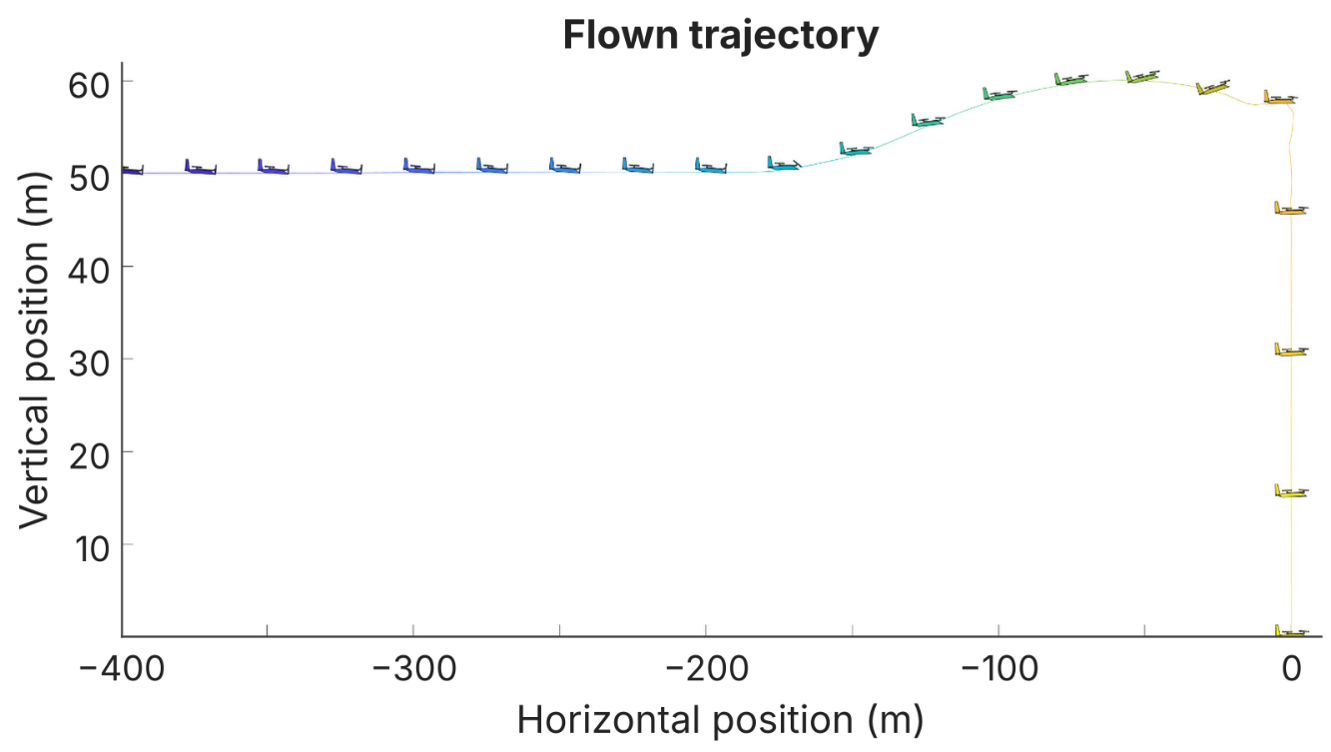
\includegraphics[width=0.8\textwidth]{images/ardupilotlanding}
  \caption{ArduPilot Landing Approach}
  \label{fig:ardupilotlanding}
\end{figure}

The transition from hover to fixed wing flight has been extensively studied as there is a much greater risk for instability of the systems as the aircraft is in a lower energy state leading to unrecoverable stalls. The transition from fixed wing flight to hover is less studied as there is a obvious and stable solution of reconfiguring the aircraft for hover while coasting in fixed wing cruise. This is the approach used in current solutions such as ArduPilot. However this approach results in extensive time spent in hover, a substantially more power intensive flight mode compared to fixed wing flight (ref Figure \ref{fig:Landing Approach Power}), as the active rotors have to counteract the gravitational force rather than the passive wings. The obvious solution of descending quicker in hover to minimise time spent in that mode has its own issues, primarily entering the vortex ring state. A phenomenon where if  a rotor powered aircraft descends at a comparable rate to the downwash velocity produced by the rotor, large vortices can form centered around the mid point of the rotor blade span and cause a dramatic loss in lift \cite{cantrell_settling}.
 

\begin{figure}[htbp]
  \centering
  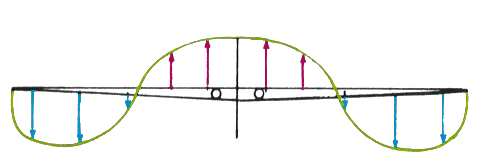
\includegraphics[width=0.8\textwidth]{images/VRS}
  \caption{Vortex Ring State Air Flow}
  \label{fig:vrs}
\end{figure}


\section{Transition Control}
\label{sec:lit_control}

The simplest approach to transition control, and the one used by most open-source autopilots, is a scheduled transition, where the tilt angle and control transition are blended as functions of airspeed or time and the attitude is stabilised by PID loops \cite{ardupilot_quadplane}. This approach is robust and simple to tune, but it is not optimal with respect to energy consumption.

Model-based controllers have already been employed to optimise these transitions. Allenspach and Ducard \cite{allenspach2021nmpc} applied model predictive control (MPC) to a tilt rotor UAV, and achieved one unified controller for all stages of flight. Ducard and Allenspach \cite{ducard2021review} propose that this single controller approach should be the direction the field moves in, along with the need to manage control complexity against the computing resources available on board, as this is a significant constraint for MPC, which requires an optimisation problem to be solved in real time on board the aircraft's flight controller, and is a primary motivation for the precomputed controller used in this project.

Learning based approaches have also been applied. Fu et al. \cite{fu2023saferl} used safe reinforcement learning for the back-transition of a ducted fan tail-sitter, minimising altitude change and transition time subject to a vertical velocity constraint, and showed that the learned trajectory closely matched the optimal trajectory obtained with GPOPS-II.

\section{Optimal Control}
\label{sec:lit_trajopt}

Trajectory optimisation refers to methods that find the control inputs which take a dynamic system between two states while minimising a cost function and satisfying the associated constraints. Direct methods transcribe this infinite dimensional problem into a finite dimensional nonlinear program (NLP) by discretising the states and controls through time. Hargraves and Paris \cite{hargraves1987direct} introduced direct collocation, in which the system dynamics are enforced as equality constraints between discrete points, and Betts \cite{betts1998survey} summarises the numerical methods used to solve such problems.

Kelly \cite{kelly2017introduction} provides a method on direct collocation, covering trapezoidal and Hermite--Simpson collocation, initialisation, and mesh refinement, and released the MATLAB library OptimTraj \cite{kelly2022optimtraj} that implements these methods; OptimTraj is the library used in this project. Kelly notes that the NLPs produced by transcription are generally non-convex, so the solver returns a locally optimal solution which depends on the initial guess. The straight line initialisation and successive mesh refinement described in Section \ref{sec:trajopt} are intended to manage this.

Trajectory optimisation has been applied to the transition problem by several authors. Naldi and Marconi \cite{naldi2011optimal} formulated minimum-time and minimum-energy transition manoeuvres for a class of V/STOL aircraft as mixed-integer nonlinear programs. Zhao et al. \cite{zhao2023multimode} computed a transition corridor (map of feasible states based of tilt angle and velocity) for a tilt rotor UAV and solved the transition strategy as a constrained optimal control problem, with a cost function built on transition time, attitude stability and control continuity. Deng et al. \cite{deng2025pigeon} extended static transition corridor to a dynamic one allowing for the aircraft to be in not be in equilibrium as well as adding angle of attack to form a three dimensional space of feasible states. Both of these approaches support modelling exclusively the longitudinal dynamics of the aircraft due to the symmetry of the airframes.
The other common factor of these two papers is the exclusion of stalled states from the trajectory, as they don't model post stall dynamics, and they lie outside the feasible states for the aircraft.

\section{Post-Stall Manoeuvring and Perching}
\label{sec:lit_perching}

The optimal trajectory found in this project dives to convert potential energy into kinetic energy, then pulls up into a stall, using the drag at high angle of attack to dissipate the majority of the aircraft's kinetic energy. This manoeuvre resembles that of perching birds, which has been studied in the context of fixed wing UAVs.

Cory and Tedrake \cite{cory2008experiments} demonstrated a fixed wing glider performing a perching manoeuvre using a model identified from motion capture data and a trajectory optimised for the post-stall regime, stabilised with a time-varying LQR. Moore, Cory and Tedrake \cite{moore2014robust} extended this work using LQR-Trees, a feedback motion planning method built on time-varying LQR around nominal trajectories, and achieved a 95\% perching success rate over 147 flights on real hardware across a wide range of initial speeds. Their results show that post-stall manoeuvres can be executed reliably with a simple airframe and a model based controller, without complex dynamic wings, at least in the absence of significant wind gusts.

These works establish that deliberately stalling an aircraft is a viable way to dissipate energy, and that time-varying LQR about an optimised trajectory is a suitable way to stabilise it. The tilt rotor in this project has an advantage over the glider in that the rotors provide control authority that is independent of airspeed, which is used to stabilise the stall in the final stage of the approach.

\section{Trajectory Tracking with Time-Varying LQR}
\label{sec:lit_tvlqr}

The linear quadratic regulator (LQR) minimises a squared cost on state error and control effort, with the optimal gain given by the solution of a Riccati equation \cite{anderson1990optimal}. For a time-varying system linearised about a trajectory over a finite horizon, the gain is found by integrating the differential Riccati equation backwards in time from a terminal condition, which produces a time-varying gain matrix  \cite{anderson1990optimal, tedrake2010lqrtrees}. As the horizon is finite, the gains reduce towards the end of the trajectory as the remaining cost of a state error becomes small relative to the control cost. This explains the reduction in gain seen near the end of the approach in Figure~\ref{fig:LQR Rotor Gains}. The weighting matrices are commonly chosen using Bryson's rule \cite{bryson1975applied}, where each diagonal weight is the inverse square of the maximum acceptable value of the corresponding state or input.

Time-varying LQR (TVLQR) should be distinguished from classical gain scheduling, where independent controllers are designed at a set of frozen operating points and interpolated as a function of a scheduling variable such as airspeed \cite{rugh2000research}. Rugh and Shamma \cite{rugh2000research} note that stability at each frozen operating point does not in general guarantee stability of the scheduled system, unless the scheduling variable changes slowly. The same caution applies to the frozen time eigenvalues of a time-varying closed loop system, so the stability of the controller in this project is also assessed along the trajectory as a whole rather than from the frozen time eigenvalues alone.

TVLQR is well suited to embedded implementation because all of the computation is done offline, and the onboard controller only needs to look up a gain and compute a matrix vector product each cycle. This is in contrast to MPC, and is the reason it was selected for this project.

\section{Rotor Aerodynamics in Non-Axial Flow}
\label{sec:lit_rotor}

When a rotor operates with a component of the freestream perpendicular to its axis of rotation, the advancing blade sees a higher airspeed than the retreating blade, producing an in-plane force opposing the motion (the H-force) and blade flapping, as described by momentum and blade element theory \cite{leishman2006principles}. Martin and Salaün \cite{martin2010true} showed that this rotor drag is significant even on small multirotors at low speed. Mahony, Kumar and Corke \cite{mahony2012multirotor} include blade flapping and induced drag in their tutorial model of multirotor dynamics, and Bangura and Mahony \cite{bangura2017thrust} used momentum theory to model rotor thrust for multirotor control. Faessler et al. \cite{faessler2018differential} showed that modelling rotor drag explicitly, rather than treating it as an unknown disturbance, significantly reduces the trajectory tracking error of a quadrotor.

The optimal trajectory in this project uses the rotors in this way, with the aircraft's velocity perpendicular to the rotor axes during the stall, so that rotor drag contributes to dissipating the kinetic energy. The public release of the ArduPilot simulator does not model this force, which motivated the rotor model developed in Section~\ref{sec:rot_model}.

\section{Implementation on Open-Source Autopilots}
\label{sec:lit_ardupilot}

ArduPilot is an open-source autopilot that supports tilt rotor and other powered lift VTOL aircraft through its QuadPlane firmware \cite{ardupilot_quadplane}. It provides a Lua scripting environment that allows custom scripts to read the vehicle state and override the outputs to the servos and motors without modifying the firmware \cite{ardupilot_lua}, and a software in the loop (SITL) simulator that runs the unmodified flight code against a simulated aircraft \cite{ardupilot_sitl}. Together these allow a controller to be deployed on an existing flight controller of a production aircraft and tested in simulation first, which is the approach taken in this project. The limited memory and processing available to the Lua environment are the main constraints on the controller, and motivate both the choice of TVLQR and the reduction in the number of stored gain matrices described in Section \ref{sec:lqr_gains}.

The accuracy of any model based controller depends on how closely the aerodynamic model matches the real aircraft. The aerodynamic coefficients of the model in this project were re-estimated from flight logs of the Griffin Pro, following the established approach of aircraft system identification from flight data \cite{klein2006aircraft}.

\section{Summary and Research Gap}
\label{sec:lit_gap}

The literature shows that the transition of powered lift VTOL aircraft has been approached through scheduled PID control, model predictive control, reinforcement learning, and trajectory optimisation within a transition corridor. The majority of this work focuses on the forward transition, constrains the aircraft to near trimmed flight, and optimises for smoothness, time and attitude rather than energy. Separately, the perching literature shows that post-stall manoeuvres can be stabilised reliably with time-varying LQR, and the multirotor literature shows that rotor drag in non-axial flow is a significant force that can be modelled and exploited.

No work was found that combines these to find an energy optimal back-transition for a tilt rotor that uses both the post-stall drag of the wing and the in-plane drag of the rotors, and implements it on an unmodified production flight controller. This thesis addresses that gap by optimising the back-transition of the Griffin Pro for minimum rotor energy, tracking it with a TVLQR implemented in ArduPilot's Lua environment.